\chapter[Model Implementation]{Model Implementation}
\label{appendix-model-implementation}


\section{Parameter values}
It is convenient to set up the model using initial values that are close to equilibrium values It is also helpful if the values are somewhat "realistic" to allow us develop an intuitive feeling for whether  model behaviour  is plausible. 

We have to do some initial calculations because we want to start near the equilibrium value. 



Basic values that have to be chosen because they are used in calculating other values are
\begin{description}
\item  [subsistence wage] $\phi$=  \$40.000 %  that is within range of resonable subsistance wage in canada for after-tax income.
\item  [width=height] extent of the city--number of lot to the margin 
\item [seed population] We need to seed it with an initial population at the center that anchors the population. cities aren't unseeded.  Zero if possible, but it is something to adjust to get reasonable behaviour
\item  [density ] worker per lot. (This give us population)
\item  [wage premium] ratio, 0.04--0.30 
\item [worker share of urban agglomeration surplus] 
WS =1 

Calculate/count baseline population 
% $N=density* width*height$
% $N=density * f * f$
$N=density * f * f  + town\_population$

Calculate  equilibrium wage premium = $1+wage\_premium ratio * \phi$

Calculate equilibrium cost of transportation c = $\omega/width$

Define the urban agglomeration surplus as $A(N^\beta-N)$.
 
\item  [$\alpha'$ ]  elasticity of output with respect to capital for a single firm. 0.18
\item  [$\beta'$ ]  elasticity of output with respect to labour for a single firm.  0.72

Calculate the output of the typical rural firm. This is done below for a firm with 100 workers and a marginal product of labour of $\phi$. I get \$20 million.

\item  [$\beta$ =1.12] Urban agglomeration coefficient: elasticity of URBAN output with respect to population 

Calculate the urban scale coefficient 
\[A = \frac{wage\_premium}{WS(population^{\beta-1}-1)}\]

(This relies on defining the surplus as $A(N^\beta-N)$.)

\end{description}


Several relationships constrain parameters if the model is near an equilibrium path. 
\begin{enumerate}
    \item From the urban model, the extent of the city is determined by transportation costs:   $\omega =c*width$.  Only two of these parameters can be set independently.

    \item From the urban model population is determined by arean and density   $N=density* width*height$. we assume the city is symmetric, so $Width=height$ and we assume plots  of land are identical, so  - $area=width*height$. Only two of height, desity and N can be set independently.  

    \item From the scale literature $Y=AN^\beta$ This establishes a relationship between urban GDP and population, which we intitially make equal to the workforce. 

    \item From neoclassical distribution theory, the equilibrium competitive labour share of output is $\beta'$
    
    \item From the urban model the urban wage is the subsistence wage plus the urban wage premium $\omega+\phi$ 

    \item From neoclassical distribution theory, the equilibrium competitive labour wage is the marginal product of labour. This should hold both in the urban and rural economies. $\omega$ is therefore the difference in the marginal productivities of labour between urban and rural, ${MPL^uMPL^R}$ .  This implies that if we set the subsistence wage, $\omega$ is constrained to satisfy \[\frac{\omega+\phi}{\phi}= \frac{MPL^U}{MPL^R}\] 
    
    \item Using a Cobb-Douglas production function, we can get explicit expressions for the marginal productivities of labour and capital. We can do this for a model rural firm to get firm-level parameters:
    \begin{quotation} \color{orange}
        We want the marginal product of labour in the rural economy at the firm level to be at least close to \$40,000.  We can create a generic rural firm and then consider an urban firm with agglomeration effects to get the parameters we need. 

Firm employment $L$ is small relative to  urban employment {N}. Assume it is 100 workers. 

Assume that the rural production function is 
\[Y^R=A^R K^\alpha L^\beta\]
where $\alpha=0.18$  and $\beta=0.761$.\footnote{These values give uys diminishing marginal product at the firm level and factor shares of 0.8 and 0.2 as required. The tricky point is that factor share are $\frac{\alpha}{\alpha + \beta}$ and $\frac{\beta}{\alpha + \beta}$. }  The marginal products pf labour and capital are 
\[MPL=\beta Y/L=\$40,000\] and\[\ MPK=\alpha Y/K =0.05\]
From the first, 

\[Y=\frac{L*\phi}{\beta}=\frac{L*\$40,000}{0..72}=\$5.555\ million\]
This is firm revenue. From the MPK, 

\[K=  \frac{\alpha Y }{r}=\frac{0..18 \$.5555\ million}{0.05} =\$20\ million \]

We now have the capital, labour and output for a model firm with a marginal product of labour  equal to the subsistence wage we have chosen. We can calculate the Scale coefficient 
\begin{equation}  
A^R= \frac{Y}{K^\alpha L^\beta}=\frac{5,000,000}{20,000,000^\alpha 100^\beta}\label{eqn-AR}\end{equation} 
So $A^R$ can be computes using equation~\ref{eqn-AR}


We now consider that this firm operates in the city and enjoys  urban agglomeration benefits. The value of the  marginal product of labour must rise to $\phi+\omega$. We to know  the urban wage premium that is consistent with the subsistence wage. Papageorgiou \cite{papageorgiouOccupationalMatchingCities2022} found a 4.1\% premuim. D'costa and Overman   show that working in London is associated with a 35.5\% higher wage than working in a rural area. The comparable figures are
10.6\% for big cities and 8.3\% for small cities and an elasticity of
wages with respect to city size of 1.6\%.. Estimates of the premium are lower  when they control of individual characteristics.   



If the $ scale\ coefficient=1.12$, $\omega$ would be $1.12*\phi$, or $4,800$. 


This supports an urban wage premium of $\omega\$8,000$.

We need to have a population size or a number of firms with a firm size. Assume the population is 10,000 and firms still have 100 workers. (All firms will have the same marginal product of labour in a competitive labour market, so size should not matter.)

\[Y^U=A^R N^\gamma K^\alpha L^\beta = N^\gamma Y^R\]
where $N^\gamma$ represents the agglomeration effect. The marginal product of labour is 
\[MPL^u=\$44,800=N^\gamma \beta Y^R/L=N^\gamma *\$40,000\]
so $N^\gamma= 1.2$ and $\gamma = \frac{log(1.12)}{log(10,000)} =.012$. 


This value is consistent with an empirical  value for  the agglomeration exponent of $\beta =  1.012$. The value is much lower than empirical estimates. Furthermore, if we consider the same firm structure and a population of one , the value falls, which suggests that agglomeration effects are not scale-independent, but instead increase with urban size. $\beta$ may itself be a function of $N$.

A second interesting possible implication of our calculation is that only part of the agglomeration effect appears in wages. Urban rents  are large, but agglomeration effects are much larger.

\hspace{-1cm}
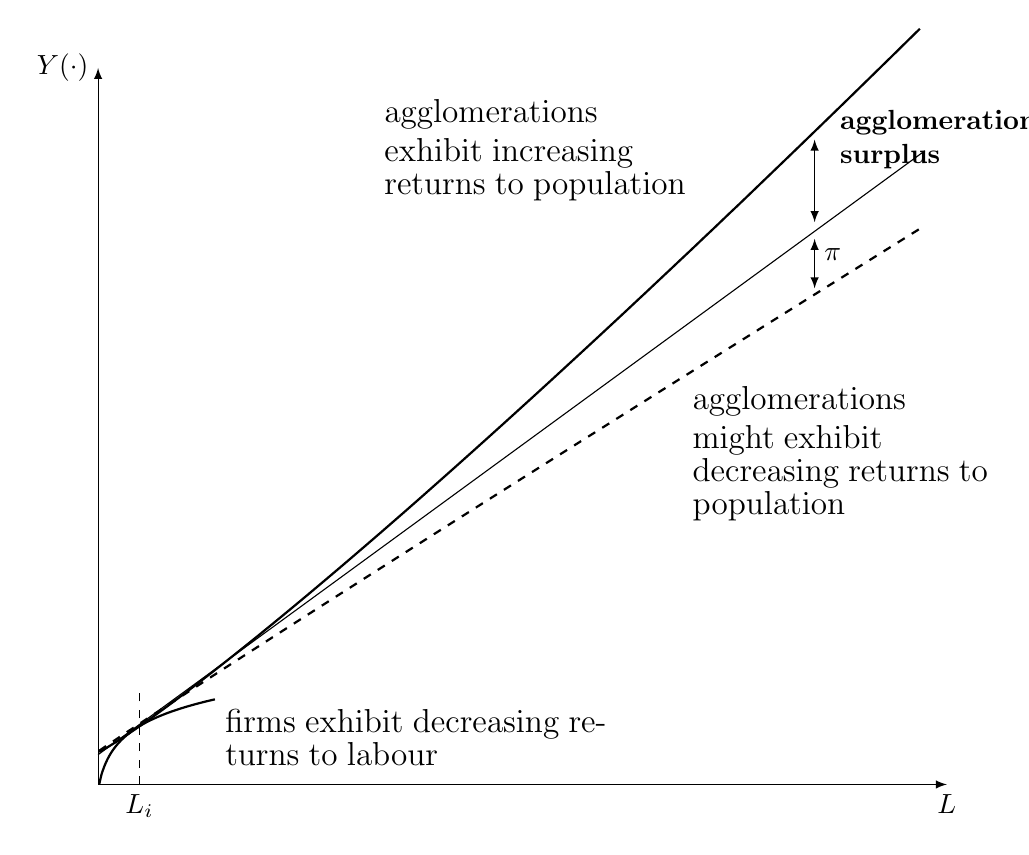
\begin{tikzpicture}[scale=.7, my plot/.style={thick, smooth, samples=100, domain=0.1:2.2},
plot2/.style={thick, smooth, samples=100, domain=0.1:14.99},
                    my grid/.style={dashed,opacity=0.5, every node/.style={black,opacity=1}},
                    my axis/.style={latex-latex}]
 
 \draw[my axis] (0,13)node[left] {$Y(\cdot)$} --(0,0)-- (15.4, 0) node[below] {$L$}; %creates the axis a little 

\coordinate (origin) at (0,0);
\def\x{0.45}
\def\y{2.1}
\def\b {$15/(2*ln(\y)+.05)$};
%\def\p{0.55} % define the x, y and p )(midpointvalues
%\draw[my plot] (0,0) plot (\x,{ln(\x)});  %Draws curve
%\draw[my plot] (0,0) plot ({\x-.08},{2.3+ln(\x)}); 
\coordinate (Uy) at (\y,{2*ln(\y)+.05});

\draw [](0,.54)--(15, 11.49625);   %diagonal. line

\draw[plot2] (0,0) plot ({\x-.08},{(\x/1.5)^1.12+.54});
\node at (11.8,11.5) [left, text width=4.5cm]{\large agglomerations\\ exhibit increasing\\ returns to population};
\draw[latex-latex] (13, 11.7)node [right=.2cm, text width=1.5cm]{\textbf{agglomeration surplus}}--(13, 10.2);
\draw[latex-latex] (13, 9)--(13, 9.9)node [below right, text width=1.5cm]{\textbf{$\pi$}};

\draw[plot2, dashed] (0,0) plot ({\x-.08},{(\x/1.5)^0.98 +.54});
\node at (13.5,6)[text width=3.8cm]{\large agglomerations might exhibit \\decreasing returns to population};

\begin{scope}[ yscale=.5,xscale=1]% shift={(1.9,0)} ,
	\coordinate (Uy) at (\y, {2.3+ln(\y)});
	\draw[my plot] (0,0) plot ({\x-.08},{2.3+ln(\x)})node[below right, text width=5.5cm]{\large firms exhibit decreasing returns to labour}; 
	\draw[dashed](.75, 0)node[below]{$L_i$} --(.75, 3.4);
\end{scope}
%
%
%\begin{scope}[shift={(1.9,0)}]
%
% \def\x{0.45}\def\y{2}\def\p{0.55} % define the x, y and p )(midpointvalues
%\draw[my plot] (0,0) plot (\x,{ln(\x)});  %Draws curve
%
%\coordinate (start plot) at (0.6,{ln(0.16)}); % domain start
%\coordinate (end plot) at (10,10); % domain end
%%\draw[my axis] ([shift={(-0.5cm,0.5cm)}]start plot |- end plot) node[left] {$Y(\cdot)$} |- node[coordinate](origin){} ([shift={(0.5cm,-0.5cm)}]start plot -| end plot) node[below] {$L$}; %creates the axis a little 
%
%\coordinate (Ux) at (\x,{ln(\x)}); % set the u(x) coordinate on the curve. Not used
%\coordinate (Uy) at (\y,{ln(\y)}); % set the u(y) coordinate on the curve
%
%\draw [](origin)--(Uy)  ; 
%
%\draw[my grid] (Uy) |- node[below]{$L*$} (origin) |- node[left]{$Y^*$} cycle;%below from on curve, the 
%
%\end{scope}

\end{tikzpicture}

    \end{quotation}

    

  

    
    

    \end{enumerate}



From the production function  $Y=Y_0N^\beta$.

Tørsløv et al \cite{torslovMissingProfitsNations2023} show that affiliates of foreign multinational firms are an order of magnitude more profitable than local firms in a number of low-tax countries. Leveraging this differential profitability, thgey estimate that 36\% of multinational profits are shifted to tax havens globally. US multinationals shift twice as much profit as other multinationals relative to the size of their foreign earnings.

\renewcommand{\sfdefault}{phv}

\section{Initial values for  the agglomeration parameter}
A segment is now redundant and has been commented out

\vspace{5lines}

% {\Large  $Prefactor = 1506.712$ based on width=height=10 and density=100} and agglomeration\_coefficient= 1.2,
% We need to get the scales of the parameters and the population size roughly consistent.

% I assume the 10X10 grid is full. 

% \section{Computing the prefactor: details}
% We have set the subsistence\_wage to \$40,000.

% The urban wage premium is in the range of 13-20\%  Assume 20\% and we get \$8,000

% Under the neoclassical assumption  \$40,000 is the  marginal productivity of rural worker

% The urban production function is 
% \[Y=AN^\beta\]
% \[Y=prefactor*working\_population**scaling\_exponent\]

% where $working\_population = width*height*density$ 

% so 
% \[Y=prefactorA*(width*height*density)^{\beta}\]

% We have more conditions that this has to satisfy: The marginal product must be consistent with the urban wage and the distribution rule. The wage cannot add up to more than total output output. Workers cannot get 1.2Y/N, for example. With CRS they would get 0.8Y/N.    

% \subsection{approach one: from agglomeration surplus}
% \[urban\_wage= subsistence\_wage + wage\_share * agglomeration\_surlpus\]
% The \textbf{agglomeration surplus} is the excess relative to the CRS case when $\beta=1$:
% \[agglomeration\_surplus= A(N^{1.2} -N^1) \]
% The urban wage premium is then the share for each worker:
% \[\omega= wage\_share * \frac{agglomeration\_surlpus}{N}\]

% and this becomes
% \[\omega= wage\_share * A\left(\frac{N^{1.2}-N^1}{N}\right)=1 * A\left(N^{0.2}-1\right)\]

% To see what this looks like, consider a population of 10,000 when  wage\_share=1
% \[\omega= \$8,000 = A\left( 6.309-1 \right)\]

% {\Large So $A = 1506.712$ based on width=height=10 and density=100}  

% Smaller N makes A bigger

% % Say width=height=15 and density= 200:
% % \[\omega= \$8,000 = A\left(10000-1\right)\]

% \subsection{Approach 2: from Marginal product and subsistance wage}
% % We want the marginal product of labour in the rural economy at the firm level to be at least close to \$40,000.

% % Firm employment $L$ is small relative to  urban employment {N}.  We can create a generic rural firm and then consider an urban firm with agglomeration effects to get the parameters we need. 

% % Assume that the rural p[rooduction function is 
% % \[Y^R=A^R K^\alpha L^\beta\]
% % where $\alpha=0.2$  and $\beta=0.8$. The marginal products are 
% % \[MPL=\beta Y/L=\$40,000\] and\[\ MPK=\alpha Y/K =0.05\]
% % From the first, 

% % \[Y=\frac{L*\$40,000}{0.8}=\$5\ million\]

% % This is firm revenue. From the MPK, 

% % \[ \frac{0.2 \$5\ million}{0.05}=K =\$20\ million \]

% % We now have the capital, labour and output for a model firm with a marginal product of labour  equal to the subsistence wage we have chosen.

% % We now consider that this firm operates in the city and enjoys  urban agglomeration benefits.  If the scale coefficient=1.12$,$ $\omega$ would be as a first appr Say that the marginal product rises to \$48,000. This supports an urban wage premium of $\omega\$8,000$.

% % We need to have a population size or a number of firms with a firm size. Assume the population is 10,000 and firms have 100 workers. All firms will have the same marginal product of labour in a competitive labour market, so size should not matter. 

% % \[Y^U=A^R N^\gamma K^\alpha L^\beta = N^\gamma Y^R\]
% % with a marginal product of 
% % \[MPL^u=\$48,000=N^\gamma \beta Y^R/L=N^\gamma *\$40,000\]
% % so $N^\gamma=1.2$ and $\gamma = .019$. 


% This value is consistent with an empirical  value for $\beta$   1.02. The value is lower than empirical estimates. Furthermore, if we consider the same firm structure and a population of one million the value falls, which suggests that agglomeration effects are not scale-independent, but instead increase with urban size. $\beta$ may itself be a function of $N$.

% A second interesting possible implication of our calculation is that only part of the agglomeration effect appears in wages. Urban rents  are large, but agglomeration effects are much larger.


 

% %\[subsistance_wage= MPL(\beta=.= \]
 % bbbb{appendix-05-agglomeration model}

\begin{lstlisting}
"""Combining a labour market and land market.

:param width: Width of the spatial grid. Each property ocupies one unit.
:param height: Height of the spatial grid. Each property ocupies one unit.
:param density: **** workers per grid cell
:param population: **** width*height*density.    #.  ****

:param transport_cost_per_dist: The cost of traveling a distance of one
    grid space. :meth:`transport_cost` cacluates travel costs using
    euclidean distance.
    
:param subsistence_wage: The value of the subsistence wage which workers
    could achieve working in the countryside. Workers will work in the
    city if it offers a wage premium above this subsistence wage.
:param working_periods: The number of time steps from when a worker
    begins work till retirement.
:param savings_rate: **** The share of the subsistence wage and net rent a worker can save in each time step, with undifferentiated labour and a uniform savings rate.


:param init_wage_offer: Initial urban wage offer. TODO consider replacing
:param init_interest_rate: TODO make this prime interest rate? YES

:param prefactor: Multiplier for the wage aglomeration effect 
:param agglomeration_ratio: Exponent for the aglomeration wage.
:param wage_share: Share of the agglomeration effect that goes to workers.
:param property_tax_annually: Property tax rate.
:param mortgage_period: The period for the mortgage. Number of years.
:param housing_services_share: Share of subsitence wage going to housing services, a.
:param maintenance_share: Share of housing services going to maintenance and sevices, b.

:param r_prime: **** BANK RATE ????  Expected return on alternative investments.
:param r_alt: **** Expected return on alternative investments.
:param r_premium_person: Person's desired return over and above 
alternative investments.
:param r_premium_bank: Bank's desired return over and above alternative investments

TODO wage should have an adjustment rate

TODO update for new parameter values, prefactor, scaling factor etc
"""
\end{lstlisting}

% For some variables, we choose arbitrarily starting values that seem resonable, because that makes it possible to check that variables that follow from computation also seem resonable, as a kind of informal sanity check.

\begin{enumerate}
\item To start with a population of around 10,000, we begin with width = 10, height = 10 and \textbf{density} per unit of 100. 

\item If we arbitrarily assume an initial wage premium around 20\%, and wish to start near equilibrium, % bettencourt assumed aggomeration exponent is indepent)
we can select transportation costs. A transportation cost of 0.1  would give a distance of $\omega/.01$, which is huge. Could this be 1/10 of the starting wage premium $\omega_0$? It would then be \$800 per year, per unit distance and would give us height and width of 10. 
% (divide into omega) - we want to start close to equilibirum. omega/cost = width
\item We should have a wage premium of about \$8000 to be consistent with the subsistance wage. % since we are assuming the wage premium of around 20%. Total wage has to be subsistence wage + wage premium, think of an average rural subistance wage seems like 45K .. 

\item Your proposed prefactor was 0.2,  251. It should be very large, based on the above numbers and the consistency constraints. I get 1507 in appendix-05-agglomeration model

\item Teminology: Y=prefactor*N**scaling\_exponent

\end{enumerate}

\begin{lstlisting}
def __init__(self, width = 50, height = 1,  # ****
             transport_cost_per_dist  = 0.1,    # c   ****
             subsistence_wage         = 40000. # psi
             working_periods          = 20,     # in years ****
             savings_rate             = 0.2, ****
            #  initial_savings: if agents save anything before reaching working age
             init_wage_offer          = 10.,  #. Makes no sense  ****
             init_interest_rate       = 0.05,

             #AGGLOMERATION MODEL features  -20% wage premium over subsistence wage, Y=prefactor*N**scaling exponent
             prefactor                = 0.2, # 251., ??????  ****. should be very large. I get 1507 
             # Prefactor - should be much higher than YES scaling_factor           =   # this is A scaling_exponent         =  1.13 # this is beta in LOBO. ****
             agglomeration_ratio      = 1.2,  # beta, was 
             wage_share               = 1.0,  # of agglomer3ation benefits
             workers_share            = 0.8   # emponent? in Slae models?
             property_tax_annually    = 0.04, # tau, was c
             mortgage_period          = 5.0,  # T, in years
             housing_services_share   = 0.3,  # a
             maintenance_share        = 0.2,  # b
             r_prime                  = 0.05,
             r_premium                = 0.005, ****
            #  r_premium_bank = 0.00, # TODO: heterogenous discount rates and premiums
             ):
\end{lstlisting}

\subsection{Workers share}
The worker's of the surplus, $lambda$ It might be 0.8. It is used in...

NOTE: 0.8 is the value of beta in a Cobb-Douglas, corresponding to the wage-share in production. It is the value used in Lobo et al

\section{Urban wage premium}

$\omega$ is the urban wage premium. It is a share of the urban agglomeration effect. 

I think of this as worker income, $\psi + \omega + r_prime*savings$ 

The wage income  $\psi + \omega$ part has to be related to the marginal productivity of workers. The urban output function from Lobo et al \cite{loboUrbanScalingProduction2013} is  
\begin{equation}Y=AN^\beta\label{LoboEqn2}\end{equation}

Where $\beta$  is the scaling exponent, with a value of,  for example, 1.13  \`a la 
Lobo. $A$ is called the ``scale factor.''\footnote{Much of the analysis assumes scale invariance of  $A$.}  The \textbf{total urban marginal productivity of a worker} is  
\[UMPL=\beta AN^{\beta-1}=\frac{\beta Y}{N} =\]
This is not the same as the \textbf{firm-level marginal productivity of a worker}. The worker total share in Lobo et al. is \[W= (1-\alpha)Y \] 
so the individual share, which should be the competitive wage, is
\[W= \frac{(1-\alpha)Y}{N} \] 
where $(1-\alpha)=0.8$ is a common estimate. If we assume that this sets the rural wage,$\phi$, then $\omega$ has to come out of the  urban surplus per worker,

\[surp= \frac{\beta -(1-\alpha)Y}{N} \] 

 so set a fraction $\lambda$ of the surplus a, and 
 \[\omega= \lambda\frac{\beta -(1-\alpha)Y}{N}= (1.13-.8) \frac{Y}{N} \] 

 Since capital expects 0.2 as its payment and labor 0.8, the surplus available to share has to be taken out of the 0.13. The easiest formulation then is probably 
 \[\omega= \lambda(\beta -1) \frac{Y}{N} =\lambda(\beta -1) \frac{AN^\beta}{N} \] 
 

$(\beta -1)$ is agglom and  $\lambda(\beta -1)$ is the workers' share of the surplus over and above the \gls{constant returns to scale} (CRS) case.   $\lambda(\beta -1)$ is 

\begin{lstlisting}
# Firm step function updates wage, omega
def step(self):
    prefactor  = self.model.prefactor
    agglom     = self.model.agglomeration_ratio
    population = self.model.agglomeration_population
    wage_share = self.model.wage_share  
    wage_premium = wage_share * (agglom-1) * prefactor * population**agglom # omega
    self.wage = wage_premium + self.model.psi
    # k thought # self.wage_premium = (wage_share * prefactor * population**agglom)/ population # omega    
    # note surplus is: (beta - 1) * (prefactor * population**agglom)
\end{lstlisting}

Where wage share is a parameter input to the model.

\section{Bidding}
\subsection{Subjective discounting}
\begin{lstlisting}
def get_discounting(self):
    """
    Delta is the subjective individual discount factor for agent
    after one year. This will be close to ri
    A factor may be a compounded rate.
    It is the present value of one dollar in one year 
    Turns one dollar in one period into dollars of present value.
    sum_delta is sum of the infinite series 
    minus discounted infinite series after mortgage_period years
    It is the present value of annual payments from one to 
    mortgage_period years e.g. of mortgage payments or rent received
    delta_mortgage_period was called   delta_period_T
    """
    
    delta = self.r_prime # if constant 
    delta_period_1 = 1 / (1 + delta) 
    delta_mortgage_period = delta_period_1**self.mortgage_period
    sum_delta = delta_mortgage_period * (1 - delta_mortgage_period)
    # Note delta_mortgage_period is subtracted to subtract the long tail
    return sum_delta
\end{lstlisting}

Delta could also depend on wealth. For example,  use the bank rate, which is the rational rate but people who are poor typically have higher rates.  It would not change as the central bank changes r-pirme
% delta could be wealth based typically higher for poor.

\begin{lstlisting}
# A version with delta depending on wealth
wealth = self.wealth
delta =
\end{lstlisting}
 
\subsection{Maintenance costs}
\begin{lstlisting}
    def get_maintenance(self):
        """Maintenance share of property service (a*b*psi summed and discounted)
        OR IS IT TOTAL maintenance COST OVER THE MORTGAGE PERIOD?
        """
        a   = self.housing_services_share
        b   = self.maintenance_share
        psi = self.subsistence_wage
        sum_delta = self.sum_delta # CALCULATE PER PERSON
        return (a * b * psi) * sum_delta
\end{lstlisting}

\subsection{Taxes}
\begin{lstlisting}
    def get_tax(self):
        """ 
        THIS DOES NOT CHANGE WITH INCREASING WAGES?
        BUT THAT IS THE MAIN WAY TO FUND A CITY

        WHAT TO CALL THIS WEHRE DOES IT GO. WHERE DO WE USE THIS VS TAU
        Just for initialization? - warranted price. 
        Use warranted prices as initialization
        Tax costs for the mortgage period, T. 
        (Example of rate for an  multiperiod annual rate)
        tax_T= tau*(omega-c*d + a*psi) * sum_delta_T
        This is assuming taxes are paid at the end of each year for T years
        tau_T       = tau * sum_T_delta 
        #  present value of the tax rate over T years        
        """
        tau   = self.model.property_tax_annually
        omega = self.firm.wage_premium # FIXED
        psi   = self.model.subsistence_wage
        a     = self.model.housing_services_share
        c     = self.model.transport_cost_per_dist # RENAME
        d     = self.distance_from_center
        sum_delta = self.model.sum_delta # TODO - make individual  - this would have to be average discounting - THIS TAKE SUM DELTA OUT - AND PUT WITH LARGER CALCULATION.. - CACLULATE FOR A PERSON/PROPERTY COMBINATION..
        return tau * (omega - c*d + a*psi) * sum_delta
\end{lstlisting}


\subsection{TODO Warranted price}
\begin{lstlisting}
@property
def warranted_price(self):
    # USELESS PLACEHOLDER - GET CALCULATION
    return self.model.firm.wage/(self.transport_cost + 1) 
\end{lstlisting}

\subsection{TODO Maximum mortgage calculation}

\textbf{wealth-based  mortgage maximum} 
 \[max\ m_i = 9-\left(\frac{W_i}{\bar W}\right)^{0.1} \]

% **Source**: Ch:model line 580, page 87.. I have done some fiddling Wealth $W_i = P-M+S.  for i - real estate agents estimated price wealth of a property owner as assessed by the bank

\textbf{income-based  mortgage maximum} of 

\[M^{max}_Yi = \frac{0.28*(\omega+w)}{r_i}\] It is the maximum the bank will let you pay.

\textbf{Combined  mortgage maximum}
\[ M_i^Y{max} = min \{9-\left(\frac{W_i}{\bar W}\right)^{0.1}P,  \frac{0.28*(\omega+w)}{r_i} \}\]

\begin{lstlisting}
# Max mortgage
wealth = property_value - mortgage + savings
mean_weath = sum(wealth)/number_of_people

def get_max_mortgage(self, applicant):
    max_mortgage =  ...
    
    return max_mortgage
\end{lstlisting}

% wealth = property_value + 
wealth $W_i = P_e-M+S$.  

- Also need mean wealth. $\bar W$ , which you have to calculate from the sums for property values total mortgages issued, and individual savings. The bank could keep these values
- Individual borrowing rate 
$r_i = (A + B \frac{\bar{W}}{W_i})\bar r=(.1 + B \frac{\bar{W}}{W_i})\bar r$.
The value .1 can be seen as the bank's share of the prime rate set by the Bank of Canada. this is an easy place to insert that value. We should discuss this detail. An alternative is
$r_i = (0 + B \frac{\bar{W}}{W_i})(\bar r_i+ bank\ margin)$.

- Maximum M  from wealth constraint = $(9-(W_i/\bar W)^{0.1}P$
  Check if $(W_i/\bar W)0.9P$ will work. 
- Maximum M  from income = $M^{max}_Yi = \frac{0.28*(\omega+w)}{r_i}$ 
% - Maximum M  $M= min(0.28*(omega+phi)/r_i,  0.8P$,  (9-(W_i/\bar W)^{0.1}P,  \frac{0.28*(\omega+w)}{r_i}   } $


 
\subsection{Net rent based on}
Tenant willing to pay, vs what it is worth for a company to buy a property.

\begin{lstlisting}
def get_net_rent(self, property):
    """Compute the rent for a land parcel, or what someone could afford
    to pay to live there. 

    Rent depends on the urban wage premium over and above the subsistence
    wage, and on transportation costs and the distance to the
    central business district. Applies with a single wage. Adjust for
    differential urban wages.

    :param property: the land parcel to get rent information for.
    """
    a     = self.model.housing_services_share
    b     = self.model.maintenance_share
    c     = self.model.transport_cost_per_dist # RENAME
    d     = property.distance_from_center 
    tau   = self.model.property_tax_annually 
    # property_tax_rate # IS THIS FOR THE MORTGAGE PERIOD
    psi   = self.model.subsistence_wage
    omega = self.model.workers_share
    return omega - c*d - a*psi - b*a*psi - tau*a*psi
    # urban_wage = self.model.firm.wage
\end{lstlisting}


\subsection{Net rent based on ..}

\begin{lstlisting}
def get_net_rent(self, property):
    """Compute the rent for a land parcel, or what someone could afford
    to pay to live there. 

    Rent depends on the urban wage premium over and above the subsistence
    wage, and on transportation costs and the distance to the
    central business district. Applies with a single wage. Adjust for
    differential urban wages.

    :param property: the land parcel to get rent information for.
    """
    a     = self.model.housing_services_share
    b     = self.model.maintenance_share
    c     = self.model.transport_cost_per_dist # RENAME
    d     = property.distance_from_center 
    tau   = self.model.property_tax_annually 
    # property_tax_rate # IS THIS FOR THE MORTGAGE PERIOD
    psi   = self.model.subsistence_wage
    omega = self.model.workers_share
    return omega - c*d - a*psi - b*a*psi - tau*a*psi
    # urban_wage = self.model.firm.wage
\end{lstlisting}

\subsection{Max Bid}

Calculate max desired bid for an agent
\begin{lstlisting}
    def get_max_bid(self, property, bidder):
        net_rent = self.get_net_rent(property)
        r        = self.model.r_prime   
        r_target = r + self.model.r_premium
        m        = 0.8 # TODO FIX - ADD WEALTH
        # I can't do delta_T. It reads as delta_transpose to me.
        sum_delta    = self.model.sum_delta 
        p_dot    = 0.01 # TODO - estimate rate of price change
        return net_rent/((1 - m)*r_target - sum_delta*(1 + p_dot - (1 + r)*m))
\end{lstlisting}

Agent will bid the min of the desired bid or the max allowed mortgage
\begin{lstlisting}
max_mortgage = self.bank.get_max_mortgage(self)
min_downpayment = self.bank.min_down_payment_share * max_mortgage
downpayment = min(min_downpayment, self.savings)
max_allowed_bid = max_mortgage + downpayment
for sale_property in (self.model.realtor.sale_listing):
    # max_bid = self.bank.get_max_bid(sale_property, self)
    # TODO Fix
    max_desired_bid = self.model.bank.get_max_bid(sale_property, self)
    max_bid = min(max_allowed_bid, max_desired_bid)
\end{lstlisting}

\section{Negotiation Process}

Bidding.

There is a problem in that they bid on all properties as a short cut. If the number of bids structures the negotiation process, we need to limit their bids or do something much more iterative. (see above section)




\section{Individual Accounting}

\begin{lstlisting}
# FIX - NEED TO ADD THIS
# Update savings
self.savings += self.model.savings_per_step

# TODO pay costs for any properties owned
# if self.residence in self.properties_owned:
#     # TODO pay mortgage if needed pay costs
#     pass
# else:
#     self.savings -= self.rent # TODO check this is right rent
\end{lstlisting}